\documentclass{ieeeojies}
\usepackage{cite}
\usepackage{amsmath,amssymb,amsfonts}
\usepackage{algorithmic}
\usepackage{graphicx}
\usepackage{textcomp}
\usepackage{array}
\usepackage[table]{xcolor}
\usepackage{multirow}
\usepackage{multicol}
\usepackage{float}
\usepackage{hyperref}
\usepackage{amsmath}

\def\BibTeX{{\rm B\kern-.05em{\sc i\kern-.025em b}\kern-.08em
    T\kern-.1667em\lower.7ex\hbox{E}\kern-.125emX}}

\title{\fontsize{21}{25}\selectfont Predicting Vietnamese airlines' stock prices utilizing statistical, machine learning, and deep learning algorithms (2019 - 2024)}

\author{
\begin{tabular}{@{}m{0.3\linewidth}@{\hskip 0.1in}m{0.3\linewidth}@{\hskip 0.1in}m{0.3\linewidth}@{}}
\centering 1st Tran Hoang Nhat & \centering 2nd Thai Ngoc Dung & \centering 3rd Nguyen Hoang Vu \tabularnewline
\centering IS403.O22.HTCL & \centering IS403.O22.HTCL & \centering IS403.O22.HTCL \tabularnewline
\centering University of Information Technology & \centering University of Information Technology & \centering University of Information Technology \tabularnewline
\centering Ho Chi Minh City & \centering Ho Chi Minh City & \centering Ho Chi Minh City \tabularnewline
\centering \href{mailto:21522420@gm.uit.edu.vn}{21522420@gm.uit.edu.vn} & \centering \href{mailto:21521982@gm.uit.edu.vn}{21521982@gm.uit.edu.vn} & \centering \href{mailto:21522799@gm.uit.edu.vn}{21522799@gm.uit.edu.vn} \tabularnewline
\end{tabular}
}


\begin{document}

\markboth
{Author: Tran Hoang Nhat, Thai Ngoc Dung, Nguyen Hoang Vu}
{Author: Tran Hoang Nhat, Thai Ngoc Dung, Nguyen Hoang Vu}

\begin{abstract}

Stock prediction plays a crucial role in economic planning and investment decision-making. This study focuses on leveraging advanced statistical,  machine learning and deep learning algorithms to predict stock prices in the Vietnamese market, with a particular emphasis on HVN, SCS, VJC. Eight time-series models, including Linear Regression, ARIMA,  RNN, GRU, LSTM, SEMOS, Stacking and FCN, are utilized for prediction. Evaluation of these models is conducted using metrics such as MAPE, RMSE, and MSLE. Furthermore, related research on stock price prediction utilizing 8 algorithms has been examined and analyzed to demonstrate their effectivenes. The dataset spans from 01/03/2019 to 29/02/2024, and only the "Close" prices (VND) are considered for analysis. This study aims to provide stakeholders with actionable insights for informed decision-making in the Vietnamese stock market.
\end{abstract}
\begin{keywords}
    Vietnam , Stock prices , LR , ARIMA , RNN , GRU , LSTM , SEMOS , Stacking , FCN
\end{keywords}


\titlepgskip=-30pt

\maketitle

\section{Introduction}
\label{sec:introduction}

Stocks represent a vital component of Vietnam's economic landscape, serving as a cornerstone for economic development and fostering investor participation. The stock market not only facilitates capital infusion into enterprises, enabling their expansion and innovation but also serves as a lucrative avenue for investors to seek returns on their investments.

Recognizing the pivotal role of stocks in driving economic progress, our endeavor focuses on leveraging advanced statistical, machine learning, and deep learning algorithms to predict stock prices in the Vietnamese market, with a particular emphasis on Vietnam Airlines JSC (HVN), SCSC Cargo Service Corporation (SCS), and Vietjet Aviation Joint Stock Company (VJC).

There are numerous amounts of time-series models, this project uses eight time-series models to predict stock price in Vietnam: Linear regression, ARIMA, RNN, GRU, LSTM, SEMOS, Stacking, FCN.

We evaluate predictive models through a comprehensive analysis based on multiple criteria such as MAPE, RMSE, MSLE, and the results of data division methods. Through this process, we determine whether this model is good or not, which model should be used, which model should not be used to estimate stock prices, providing stakeholders with clear insights and decision-making support tools.

\section{Related Works}

Due to the profitability and importance of stocks, many methods have been developed to predict stock prices. Here, we will utilize 8 algorithms: Stacking, FCN, SEMOS, Linear regression, ARIMA, RNN, GRU and LSTM. Below are some related research papers on stock price prediction using these 8 algorithms. 

In the study by Philip Ngare, Dennis Ikpe, and Samuel Asante Gyamerah, three models were employed: AdaBoost, KNN, and Stacking (AdaBoost and KNN serve as base-level classifiers, and GBM acts as the meta-level classifier). They utilized a dataset obtained from the Nairobi Stock Exchange, and the results showed that the Stacking model outperformed the two individual models, AdaBoost and KNN. This demonstrates that combining different models using the stacking ensemble learning method can lead to better results[1]. 

In the research by Shima Nabiee and Nader Bagherzadeh, they compared the performance of six different models, including FCN, SegNet, U-Net, DeepLab V3+, and two proposed models with 20-day and 40-day input frames, respectively. The results showed that when using price frames as input, FCN performed extremely well and ranked second among the six models. Notably, when the input was changed to trends, the FCN model achieved the best results among all six models, demonstrating that FCN is very suitable for stock prediction. Additionally, it was observed that when the input frame is 1 (40 days), it provides better short-term prediction results, and when the number of input frames increases, the long-term results are improved [2].

The research of David Jobst, Annette Möller, and Jürgen Groß has shown that  SEMOS is used to enhance the forecasting performance of numerical weather prediction (NWP) models by employing finite Fourier series, making it a clearly seasonal and trend-aware time series model. The results show that SEMOS provides more accurate weather forecasts based on evaluation metrics such as CRPS, LogS, and RMSE. Additionally, SEMOS maintains good forecasting performance across different time horizons. These advantages indicate that SEMOS could be a good choice for applying to stock market forecasting[3].

In the study by Xiwen Jin and Chaoran Yi, they conducted a comparison of the effectiveness among 6 models: LSTM, GRU, RandomForest, XGBoost, LightGBM, and Linear Regression, and found that GRU yielded the best results, followed by LSTM and Linear Regression. The R2 scores were as follows: LSTM 0.84, GRU 0.86, Linear Regression 0.73, and the MSE scores were: LSTM 7.06, GRU 6.26, Linear Regression 6.64 [4]. In another research by Dias Satria, four models were employed: ARIMA, RNN, LSTM, and GRU. The results showed that GRU exhibited the best performance in predicting stock prices, followed by LSTM and RNN, while ARIMA was deemed unsuitable due to the nonlinear characteristics of the data, violating the assumption of white noise in the estimation of ARIMA Box-Jenkins parameters [5].

\section{Materials}
\subsection{Dataset}

The historical stock price of Vietnam Airlines JSC (HVN), SCSC Cargo Service Corporation (SCS) and Vietjet Aviation Joint Stock Company (VJC) from 01/03/2019 to 29/02/2024 will be applied. The data contains column such as Date, Open, High, Low, Close, Volume. As the goal is to forecast close prices, only data relating to column “close" (VND) will be processed.

\subsection{Descriptive Statistics}
\begin{table}[H]
  \centering
  \caption{HVN, SCS, VJC’s Descriptive Statistics}
\begin{tabular}{|>{\columncolor{red!20}}c|c|c|c|}
    \hline
     \rowcolor{red!20} & HVN & SCS & VJC \\ \hline
     Count & 1,245 & 1,253 & 1,252 \\ \hline
     Mean & 20,266 & 63,678 & 117,882\\ \hline
     Std & 6,462& 8,429 & 14,232\\ \hline
     Min & 8,610 & 37,320 & 93,800\\ \hline
     25\% & 13,500 & 59,500 & 105,500\\ \hline
     50\% & 21,011 & 64,629 & 117,400\\ \hline
     75\% & 25,000 & 67,350 & 129,000\\ \hline
     Max & 34,753 & 85,420 & 149,000\\ \hline
\end{tabular}
\end{table}

\begin{figure}[H]
    \centering
    \begin{minipage}{0.23\textwidth}
    \centering
    \includegraphics[width=1\textwidth]{bibliography/Figure/HVN_box-plot.png}
    \caption{HVN stock price's boxplot}
    \label{fig:1}
    \end{minipage}
    \hfill
    \begin{minipage}{0.23\textwidth}
    \centering
    \includegraphics[width=1\textwidth]{bibliography/Figure/HVN_histogram.png}
    \caption{HVN stock price's histogram}
    \label{fig:2}
    \end{minipage}
\end{figure}

\begin{figure}[H]
    \centering
    \begin{minipage}{0.23\textwidth}
    \centering
    \includegraphics[width=1\textwidth]{bibliography/Figure/SCS_box-plot.png}
    \caption{SCS stock price's boxplot}
    \label{fig:1}
    \end{minipage}
    \hfill
    \begin{minipage}{0.23\textwidth}
    \centering
    \includegraphics[width=1\textwidth]{bibliography/Figure/SCS_histogram.png}
    \caption{SCS stock price's histogram}
    \label{fig:2}
    \end{minipage}
\end{figure}

\begin{figure}[H]
    \centering
    \begin{minipage}{0.23\textwidth}
    \centering
    \includegraphics[width=1\textwidth]{bibliography/Figure/VJC_box-plot.png}
    \caption{VJC stock price's boxplot}
    \label{fig:1}
    \end{minipage}
    \hfill
    \begin{minipage}{0.23\textwidth}
    \centering
    \includegraphics[width=1\textwidth]{bibliography/Figure/VJC_histogram.png}
    \caption{VJC stock price's histogram}
    \label{fig:2}
    \end{minipage}
\end{figure}

\section{Methodology}
\subsection{Linear Regression}
Linear Regression is a method of statistical analysis used to determine the relationship between a dependent variable and one or many independent variables. It is used to predict the value of the dependent variable based on the value of the independent variables.
A multiple linear regression model has the form: 
\[Y=\beta_0+\beta_1X_1+\beta_2X_2+\cdots+\beta_kX_k+\varepsilon \quad[12]\]
Where:\\
	\indent\textbullet\ Y is the dependent variable.\\
	\indent\textbullet\ \(X_1, X_2, \ldots, X_k\) are the independent variables.\\
	\indent\textbullet\ \(\beta_0\) is the intercept term.\\
	\indent\textbullet\ \(\beta_1,..., \beta_k\) are the regression coefficients for the independent variables.\\
	\indent\textbullet\ \(\varepsilon\) is the error term.
 \subsection{ARIMA}
 ARIMA(Autoregressive Integrated Moving Average) is a statistical forecasting method widely used in time series analysis. This model incorporates autoregressive (AR), moving average (MA) and Integrated (I) components to capture the relationship between current and past values of a time series.\\
Auto Regression (AR): 
$$
y_t=\mu+\sum_{i=1}^p \gamma_i y_{t-i}+\epsilon_t \quad [6]
$$

In there : $\mathrm{y}_{\mathrm{t}}$ is the current value; $\mu$ is the constant term; $\mathrm{p}$ is the number of autoregressive terms; $\gamma_{\mathrm{i}}$ is the autocorrelation coefficient and $\varepsilon_{t}$ is error.\\
Moving Average (MA):
$$
y_t=\mu+\sum_{i=1}^q \theta_i \epsilon_{t-i}+\epsilon_t \quad [6]
$$

In there : $\mathrm{y}_{\mathrm{t}}$ is the current value; $\mu$ is the constant term; $\mathrm{q}$ is the number of terms in the moving average; $\theta_{\mathrm{i}}$ is the moving average coefficient  and $\varepsilon_{t}$ is error.\\
Integrated (I):\\
 \\$\mathrm{I}(d=0): \Delta y_t=y_t$\\
 \\$\mathrm{I}(d=1): \Delta y_t=y_t-y_{t-1}$\\
 \\$\mathrm{I}(d=2): \Delta\left(\Delta y_t\right)=\left(y_t-y_{t-1}\right)-\left(y_{t-1}-y_{t-2}\right)$ \\
 
In there : d is the number of differences required to make it a stationary sequence 

After combining them, we will have the ARIMA (p, d, q) express as follow:
$$
y_t=\mu+\sum_{i=1}^p \gamma_i y_{t-i}+\sum_{i=1}^q \theta_i \epsilon_{t-i}+\epsilon_t \quad [6]
$$
\subsection{SEMOS}
SEMOS (Smooth EMOS) is a statistical approach used for post-processing ensemble forecasts, particularly to handle seasonal variations in the predictive distribution parameters. SEMOS integrates seasonal effects directly into the estimation of location and scale parameters, enhancing the accuracy of ensemble forecasts, especially for quantities exhibiting seasonal variability.

The first parameter is location, in general, represents the central tendency or the "location" of the predictive distribution.In SEMOS, the location parameter is modeled as a function of the ensemble mean forecast and seasonal effects in order to capture systematic biases or trends in the ensemble forecasts:
$$
\mu_S(t) = a_0 + f_0(t) + (a_1 + f_1(t)) . x(t) \quad[3]
$$

Where: \\
        \indent\textbullet\ \(\mu_S(t)\) is the location parameter at time t. \\
        \indent\textbullet\ \(a_0, a_1\) are coefficients representing the baseline intercept and slope. \\
        \indent\textbullet\ \(f_0(t), f_1(t)\) are seasonal effects modeled using cyclic regression splines. \\
        \indent\textbullet\ \(x(t)\) is the ensemble mean forecast at time t \\

The scale parameter represents the spread or "scale" of the predictive distribution.It accounts for variations in forecast uncertainty over time, including factors such as model errors and ensemble spread, modeled as a function of the empirical ensemble standard deviation and seasonal effects.
\[log(\sigma_S(t)) = b_0 + g_0(t) + (b_1 + g_1(t)).s(t) \quad[3]\]
Where: \\
        \indent\textbullet\ \(\sigma_S(t)\) is the scale parameter at time t. \\
        \indent\textbullet\ \(b_0, b_1\) are coefficients representing the baseline intercept and slope. \\
        \indent\textbullet\ \(g_0(t), g_1(t)\) are seasonal effects modeled using cyclic regression splines. \\
        \indent\textbullet\ \(s(t)\) is the empirical ensemble standard deviation at time step t.

\subsection{Stacking}

Stacking, short for Stacked Generalization, is a machine learning algorithm belonging to the Ensemble Learning category. A basic Stacking model is usually divided into two levels: level-0 models and the level-1 model. Level-0 models (base-models) are the foundational models that learn directly from the dataset and produce predictions for the level-1 model (meta-model). The meta-model is trained based on the predicted outputs of the base models. These outputs, combined with the labels, form the input-output pairs during the training process of the meta-model. In this work, ARIMAX and RNN are used as base-models and Linear Regression is selected as meta-model.  
\begin{figure}[H]
  \centering
  \begin{minipage}{0.9\linewidth}
    \centering
    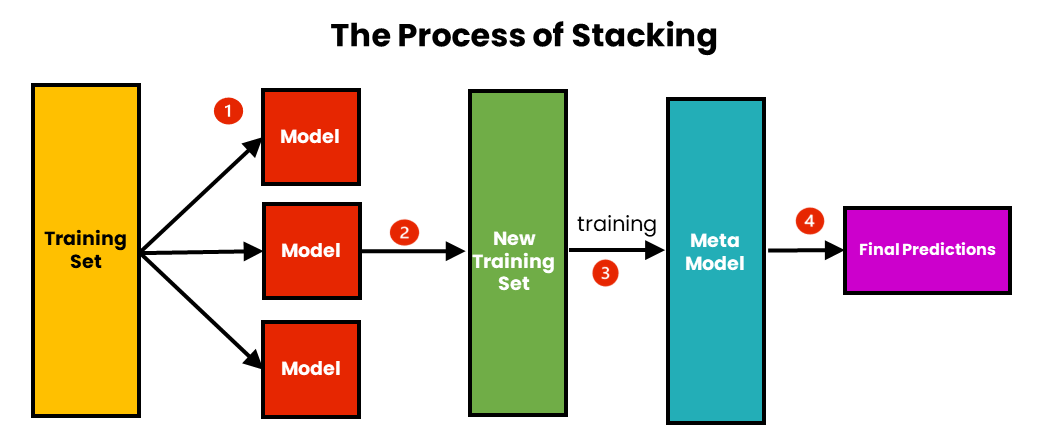
\includegraphics[width=\linewidth]{bibliography/Stacking.png}
    \caption{Stacking Architecture [7]}
    \label{fig8}
  \end{minipage}
\end{figure}


\subsection{FCN}
Fully Convolutional Neural Networks (FCNs) were first proposed in Wang et al. (2017b) for classifying univariate time series and validated on 44 datasets from the UCR/UEA archive. FCNs are mainly convolutional networks that do not contain any local pooling layers which means that the length of a time series is kept unchanged throughout the convolutions. In addition, one of the main characteristics of this architecture is the replacement of the traditional final FC layer with a Global Average Pooling (GAP) layer which reduces drastically the number of parameters in a neural network while enabling the use of the CAM (Zhou et al., 2016) that highlights which parts of the input time series contributed the most to a certain classification.  [11]
\begin{figure}[H]
    \centering
    \begin{minipage}{1\linewidth}
        \centering
        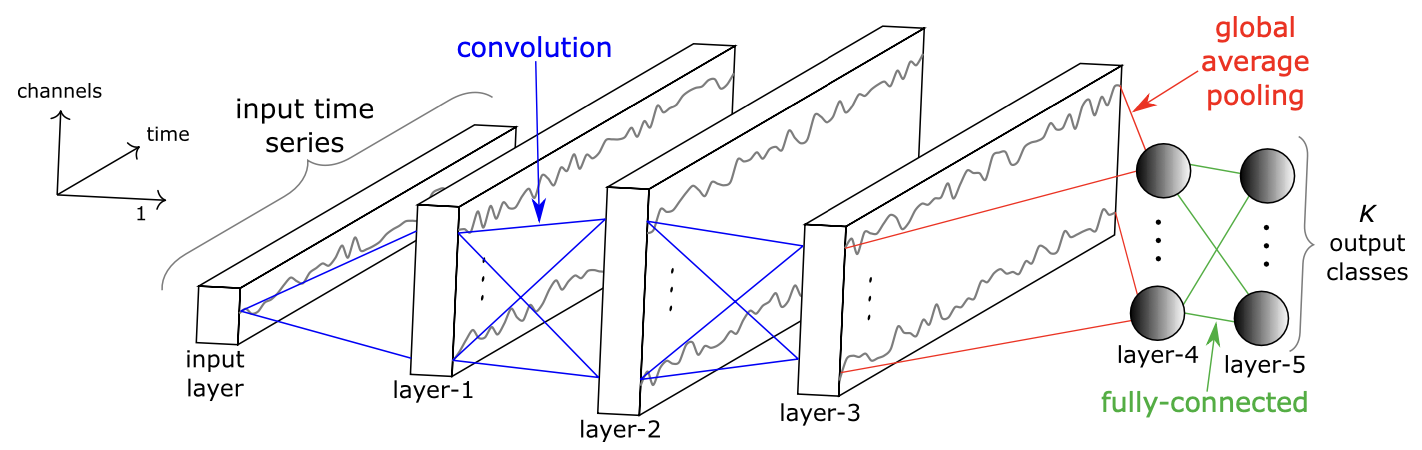
\includegraphics[width=\linewidth]{bibliography/fullyConvolutionalNeuralNetworkArchitecture.png}
        \caption{Fully Convolutional Neural Network architecture [11]}
        \label{fig11}
    \end{minipage}
\end{figure}




%% UNCOMMENT these lines below (and remove the 2 commands above) if you want to embed the bibliografy.
\begin{thebibliography}{00}
\bibitem{b1} S. A. Gyamerah, P. Ngare and D. Ikpe, "On Stock Market Movement Prediction Via Stacking Ensemble Learning Method," 2019 IEEE Conference on Computational Intelligence for Financial Engineering \& Economics (CIFEr), Shenzhen, China, 2019, pp. 1-8, doi: 10.1109/CIFEr.2019.8759062.
\bibitem{b2} S. Nabiee và N. Bagherzadeh, "Stock Trend Prediction: A Semantic Segmentation Approach,"  Mar 2023, doi: 10.48550/arXiv.2303.09323.
\bibitem{b3} D. Jobst, A. Möller, and J. Groß, "Time Series based Ensemble Model Output Statistics for Temperature Forecasts Postprocessing", Feb 2024, doi: 10.48550/arXiv.2402.00555.
\bibitem{b4} Xiwen Jin and Chaoran Yi, "The Comparison of Stock Price Prediction Based on Linear Regression Model and Machine Learning Scenarios," in Proceedings of the 2022 International Conference on Bigdata Blockchain and Economy Management (ICBBEM 2022), December 2022, pp. 837-842, doi: 10.2991/978-94-6463-030-5\_82.
\bibitem{b5} D. Satria, "Predicting Banking Stock Prices Using RNN, LSTM, and GRU Approach," Applied Computer Science, vol. 19, no. 1, pp. 82-94, March 2023, doi: 10.35784/acs-2023-06
\bibitem{b6} S. Kumar, A. Gupta, K. Arora, and K. Vatta, "Effect of Rainfall in Predicting Tomato Prices in India: An Application of SARIMAX and NARX Model" December 2022, vol. 32, no. 2, pp. 159-164
\bibitem{b7} B. Soni, "Stacking to Improve Model Performance: A Comprehensive Guide on Ensemble Learning in Python", Medium. Accessed: May 12, 2024. [Online]. Available: https://medium.com/@brijesh\_soni/stacking-to-improve-model-performance-a-comprehensive-guide-on-ensemble-learning-in-python-9ed53c93ce28
\bibitem{b8} A. Amidi and S. Amidi, "Recurrent Neural Networks cheatsheet" Stanford University. [Accessed: May 25, 2024]. [Online]. Available: https://stanford.edu/~shervine/teaching/cs-230/cheatsheet-recurrent-neural-networks
\bibitem{b9} Nguyen Minh Nhut, “Mo Hinh Mang Hoi Quy (RNN) trong chuoi thoi gian”
\bibitem{b10} Farhad Mortezapour Shiri, Thinagaran Perumal, Norwati Mustapha and Raihani Mohamed, "A Comprehensive Overview and Comparative Analysis on Deep Learning Models: CNN, RNN, LSTM, GRU", May 2023, doi: 10.48550/arXiv.2305.17473
\bibitem{b11} H. I. Fawaz, G. Forestier, J. Weber, L. Idoumghar, and P.-A. Muller, "Deep learning for time series classification: a review," Data Mining and Knowledge Discovery, vol. 33, no. 4, pp. 917-963, Jul. 2019, doi: 10.1007/s10618-019-00619-1.
\bibitem{b12} D. C. Montgomery, E. A. Peck, and G. G. Vining, "Introduction to Linear Regression Analysis," 5th ed., Hoboken, NJ, USA: Wiley, 2012.

\end{thebibliography}
%%%%%%%%%%%%%%%


\EOD

\end{document}
